\subsection{Domain Throughput Comparison}
\label{sec:resTh}

To gain a first global view, \figref{fig:th} plots the throughput improvement of the two domains over increasing HW budget.

%Graph is Average Throughput Improvement
\begin{figure}[htb]
	%\vspace{-10pt}
	\centering
		\subfloat[OpenVX Domain]{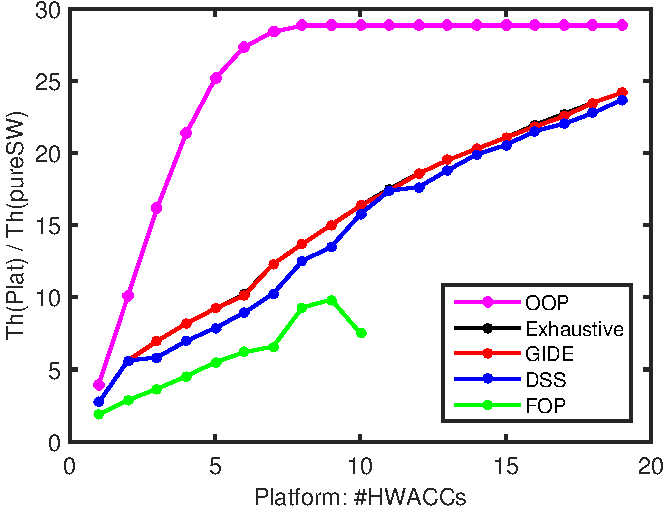
\includegraphics[width=.48\linewidth]{fig/prThOpenVX.pdf}\label{fig:thOpenVX}}
		\hfill
		\subfloat[Synthetic Domain]{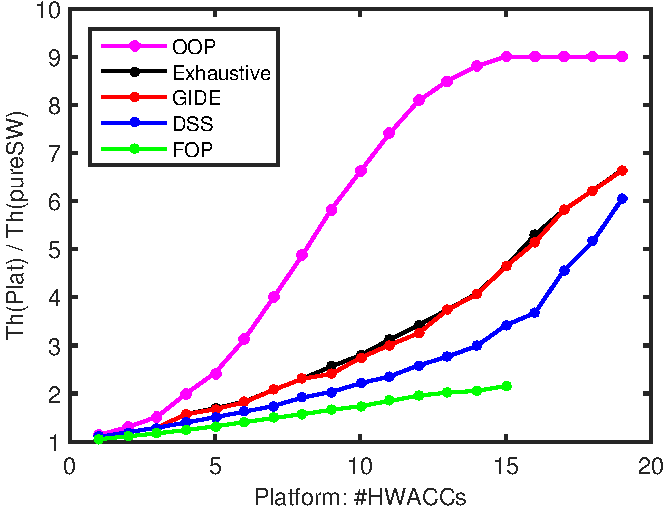
\includegraphics[width=.48\linewidth]{fig/prThSyn.pdf}\label{fig:thSyn}}
	%\vspace{-5pt}
	\caption{Average throughput improvement}
	\label{fig:th}
	%\vspace{-4pt}
\end{figure}

\textbf{OOP} yields highest (but unrealistic) throughput, see \figref{fig:thOpenVX}, assuming that each application were to execute on its own OPT. This indicates the acceleration potential. It saturates with budget $N$=10, when each application has enough accelerators. However, considering a single platform for all applications, \textbf{Exhaustive} indicates the optimum. It linearly increases with $N$ closing the gap to OOP, indicating that the additional area is well invested. \textbf{\ga} (actually \gah) almost achieves domain optimal, tracking Exhaustive. The greedy \textbf{DSS} is measurably below optimum but the gap narrows with budget. Exploring at application scope incurs dramatic penalties as indicated with \textbf{FOP} on the bottom.
FOP plateaus with 10 ACCs as already all possible ACCs have been selected for each application and it cannot outside this application to accelerate.
Comparing against FOP, \ga and DSS have 74.85\% and 58.02\% higher throughput ($N$\textless=10).

The synthetic domain, \figref{fig:thSyn}, exhibits similar trends. OOP and FOP saturate later $N$=15 due to the larger domain (more function types). Given larger domain, the gap between DSS and GA is increased. As the synthetic domain has a larger design space, the DSE performance has more impact on the results. Here, \ga and DSS have a 48.09\% and 23.60\% higher throughput ($N$\textless=15).

In order to better delineate DSE performance, we define the metric \textbf{average throughput achievement}. It scales the throughput improvement of a DSE generated platform over the throughput improvement of the domain optimal platform (i.e. Exhaustive) of the same budget. An throughput achievement of 1 thus indicates the optimum. \figref{res:pa} graphs the achievements.

%Graph is Performance Achievement
\begin{figure}[htbp]
	\vspace{-5pt}
	\centering
		\subfloat[OpenVX Domain]{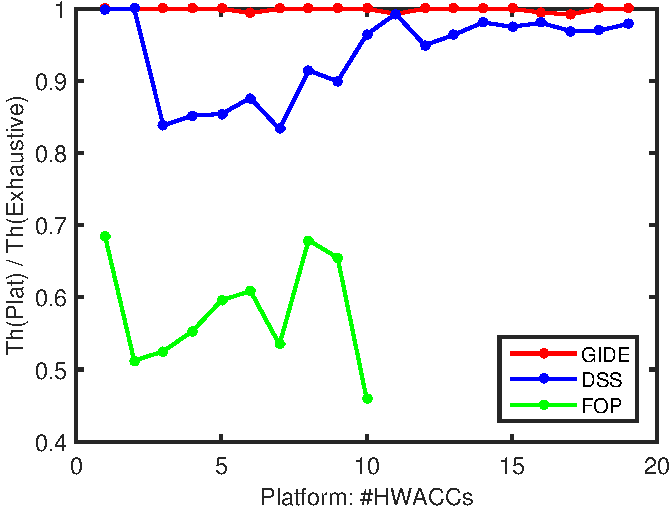
\includegraphics[width=.48\linewidth]{fig/prPAOpenVX.pdf}\label{fig:paOpenVX}}
		\hfill
		\subfloat[Synthetic Domain]{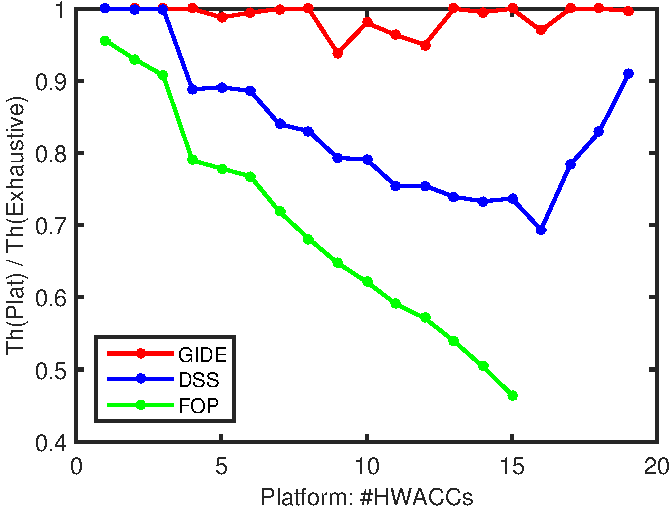
\includegraphics[width=.48\linewidth]{fig/prPASyn.pdf}\label{fig:paSyn}}
	%\vspace{-8pt}
	\caption{Average Throughput Achievement}
	\label{res:pa}
	%\vspace{-4pt}
\end{figure}

In \figref{fig:paOpenVX}, \ga achieves close to the optimum, with 99.87\% on average across all budgets for the OpenVX domain. DSS achieves less with 93.65\% and is not as stable. FOP has a large gap with only 58.07\%.

Considering the larger synthetic domain, \figref{fig:paSyn} shows even more differentiation. GA, DSS, FOP achieve 98.84\%, 83.45\% and 69.81\%, respectively. The gap between DSS and GA is more pronounced and largest gap shifts from $N$=7 in OpenVX to $N$=16 in synthetic domain. Beyond that point, DSE performance is not as critical as with a higher HW budget the margins between the ACCs selection become smaller, thus selecting a sub-optimal ACC has a lower penalty.


